\documentclass[UTF8,12pt]{ctexart}
\usepackage[a4paper,margin=24mm]{geometry}
\usepackage{amsmath,amssymb,bm,graphicx,adjustbox}
\newcommand{\fitmath}[1]{\begin{adjustbox}{max width=\linewidth}$\displaystyle #1$\end{adjustbox}}
\setlength{\parindent}{0pt}
\setlength{\parskip}{.7em}
\sloppy
\allowdisplaybreaks
\begin{document}
\section*{2015 年考研数学三 · 真题}
\subsection*{原 PDF 第 21 页}

\subsection*{2015 年全国硕士研究生招生考试试题}

\subsection*{一、选择题（本题共 8 小题，每小题 4 分，共 32 分。在每小题给出的四个选项中，只有一项符合题目要求，把所选项前的字母填在题后的括号内。）}

(1) 设 \(\displaystyle \{x_n\}\) 是数列。下列命题中不正确的是（　）。


(A) 若 \(\displaystyle \lim_{n\to\infty}x_n=a\)，则 \(\displaystyle \lim_{n\to\infty}x_{2n}=\displaystyle \lim_{n\to\infty}x_{2n+1}=a\)。 (B) 若 \(\displaystyle \lim_{n\to\infty}x_{2n}=\displaystyle \lim_{n\to\infty}x_{2n+1}=a\)，则 \(\displaystyle \lim_{n\to\infty}x_n=a\)。


(C) 若 \(\displaystyle \lim_{n\to\infty}x_n=a\)，则 \(\displaystyle \lim_{n\to\infty}x_{3n}=\displaystyle \lim_{n\to\infty}x_{3n+1}=a\)。 (D) 若 \(\displaystyle \lim_{n\to\infty}x_{3n}=\displaystyle \lim_{n\to\infty}x_{3n+1}=a\)，则 \(\displaystyle \lim_{n\to\infty}x_n=a\)。


(2) 设函数 \(\displaystyle f(x)\) 在 \(\displaystyle ( -\infty,\allowbreak +\infty )\) 内连续，其 2 阶导函数 \(\displaystyle f^{\prime\prime}(x)\) 的图形如右图所示，则曲线 \(\displaystyle y=f(x)\) 的拐点个数为（　）。


(A) 0。 (B) 1。 (C) 2。 (D) 3。


\begin{center}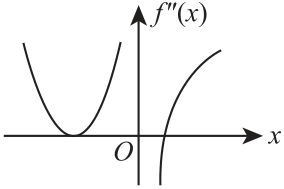
\includegraphics[width=.85\linewidth]{../assets/figures/page-021-07.png}\end{center}

(3) 设 \(\displaystyle D=\{(x,\allowbreak y)\mid x^2+y^2\leq 2x,\allowbreak \ x^2+y^2\leq 2y\}\)，函数 \(\displaystyle f(x,\allowbreak y)\) 在 \(\displaystyle D\) 上连续，则 \(\displaystyle \iint_D f(x,\allowbreak y)\,dx\,dy=\)（　）。


(A) \(\displaystyle \int_0^{\pi/4}d\theta\displaystyle \int_0^{2\cos\theta}f(r\cos\theta,\allowbreak r\sin\theta)r\,dr+\displaystyle \int_{\pi/4}^{\pi/2}d\theta\displaystyle \int_0^{2\sin\theta}f(r\cos\theta,\allowbreak r\sin\theta)r\,dr\)。


(B) \(\displaystyle \int_0^{\pi/4}d\theta\displaystyle \int_0^{2\sin\theta}f(r\cos\theta,\allowbreak r\sin\theta)r\,dr+\displaystyle \int_{\pi/4}^{\pi/2}d\theta\displaystyle \int_0^{2\cos\theta}f(r\cos\theta,\allowbreak r\sin\theta)r\,dr\)。


(C) \(\displaystyle 2\displaystyle \int_0^1dx\displaystyle \int_{1-\sqrt{1-x^2}}^x f(x,\allowbreak y)\,dy\)。 (D) \(\displaystyle 2\displaystyle \int_0^1dx\displaystyle \int_x^{\sqrt{2x-x^2}}f(x,\allowbreak y)\,dy\)。


(4) 下列级数中发散的是（　）。


(A) \(\displaystyle \sum_{n=1}^{\infty}\dfrac{\displaystyle n}{\displaystyle 3^n}\)。 (B) \(\displaystyle \sum_{n=1}^{\infty}\dfrac{\displaystyle 1}{\displaystyle \sqrt n}\ln\left(1+\dfrac{\displaystyle 1}{\displaystyle n}\right)\)。 (C) \(\displaystyle \sum_{n=2}^{\infty}\dfrac{\displaystyle (-1)^n+1}{\displaystyle \ln n}\)。 (D) \(\displaystyle \sum_{n=1}^{\infty}\dfrac{\displaystyle n!}{\displaystyle n^n}\)。


(5) 设矩阵 \(\displaystyle A=\begin{pmatrix}1&1&1\\1&2&a\\1&4&a^2\end{pmatrix},\allowbreak \ b=\begin{pmatrix}1\\d\\d^2\end{pmatrix}\)。若集合 \(\displaystyle \Omega=\{1,\allowbreak 2\}\)，则线性方程组 \(\displaystyle Ax=b\) 有无穷多解的充分必要条件为（　）。


(A) \(\displaystyle a\notin\Omega,\allowbreak d\notin\Omega\)。 (B) \(\displaystyle a\notin\Omega,\allowbreak d\in\Omega\)。 (C) \(\displaystyle a\in\Omega,\allowbreak d\notin\Omega\)。 (D) \(\displaystyle a\in\Omega,\allowbreak d\in\Omega\)。


(6) 设二次型 \(\displaystyle f(x_1,\allowbreak x_2,\allowbreak x_3)\) 在正交变换 \(\displaystyle x=Py\) 下的标准形为 \(\displaystyle 2y_1^2+y_2^2-y_3^2\)，其中 \(\displaystyle P=(e_1,\allowbreak e_2,\allowbreak e_3)\)。若 \(\displaystyle Q=(e_1,\allowbreak -e_3,\allowbreak e_2)\)，则 \(\displaystyle f(x_1,\allowbreak x_2,\allowbreak x_3)\) 在正交变换 \(\displaystyle x=Qy\) 下的标准形为（　）。


\clearpage

\subsection*{原 PDF 第 22 页}

(A) \(\displaystyle 2y_1^2-y_2^2+y_3^2\)。 (B) \(\displaystyle 2y_1^2+y_2^2-y_3^2\)。 (C) \(\displaystyle 2y_1^2-y_2^2-y_3^2\)。 (D) \(\displaystyle 2y_1^2+y_2^2+y_3^2\)。


(7) 若 \(\displaystyle A,\allowbreak B\) 为任意两个随机事件，则（　）。


(A) \(\displaystyle P(AB)\leq P(A)P(B)\)。 (B) \(\displaystyle P(AB)\geq P(A)P(B)\)。 (C) \(\displaystyle P(AB)\leq\dfrac{\displaystyle P(A)+P(B)}{\displaystyle 2}\)。 (D) \(\displaystyle P(AB)\geq\dfrac{\displaystyle P(A)+P(B)}{\displaystyle 2}\)。


(8) 设总体 \(\displaystyle X\sim B(m,\allowbreak \theta)\)，\(\displaystyle X_1,\allowbreak X_2,\allowbreak \ldots,\allowbreak X_n\) 为来自该总体的简单随机样本，\(\displaystyle \overline X\) 为样本均值，则 \(\displaystyle E\left[\displaystyle \sum_{i=1}^n(X_i-\overline X)^2\right]=\)（　）。


(A) \(\displaystyle (m-1)n\theta(1-\theta)\)。 (B) \(\displaystyle m(n-1)\theta(1-\theta)\)。 (C) \(\displaystyle (m-1)(n-1)\theta(1-\theta)\)。 (D) \(\displaystyle mn\theta(1-\theta)\)。


\subsection*{二、填空题（本题共 6 小题，每小题 4 分，共 24 分，把答案填在题中横线上。）}

(9) \(\displaystyle \lim_{x\to0}\dfrac{\displaystyle \ln(\cos x)}{\displaystyle x^2}=\)\_\_\_\_\_\_。


(10) 设函数 \(\displaystyle f(x)\) 连续，\(\displaystyle \varphi(x)=\displaystyle \int_0^{x^2}xf(t)\,dt\)。若 \(\displaystyle \varphi(1)=1,\allowbreak \ \varphi^{\prime}(1)=5\)，则 \(\displaystyle f(1)=\)\_\_\_\_\_\_。


(11) 若函数 \(\displaystyle z=z(x,\allowbreak y)\) 由方程 \(\displaystyle e^{x+2y+3z}+xyz=1\) 确定，则 \(\displaystyle dz|_{(0,\allowbreak 0)}=\)\_\_\_\_\_\_。


(12) 设函数 \(\displaystyle y=y(x)\) 是微分方程 \(\displaystyle y^{\prime\prime}+y^{\prime}-2y=0\) 的解，且在 \(\displaystyle x=0\) 处 \(\displaystyle y(x)\) 取得极值 3，则 \(\displaystyle y(x)=\)\_\_\_\_\_\_。


(13) 设 3 阶矩阵 \(\displaystyle A\) 的特征值为 \(\displaystyle 2,\allowbreak -2,\allowbreak 1\)，\(\displaystyle B=A^2-A+E\)，其中 \(\displaystyle E\) 为 3 阶单位矩阵，则行列式 \(\displaystyle |B|=\)\_\_\_\_\_\_。


(14) 设二维随机变量 \(\displaystyle (X,\allowbreak Y)\) 服从正态分布 \(\displaystyle N(1,\allowbreak 0;1,\allowbreak 1;0)\)，则 \(\displaystyle P\{XY-Y<0\}=\)\_\_\_\_\_\_。


\subsection*{三、解答题（本题共 9 小题，共 94 分，解答应写出文字说明、证明过程或演算步骤。）}

(15)（本题满分 10 分）设函数 \(\displaystyle f(x)=x+a\ln(1+x)+bx\sin x,\allowbreak \ g(x)=kx^3\)。若 \(\displaystyle f(x)\) 与 \(\displaystyle g(x)\) 在 \(\displaystyle x\to0\) 时是等价无穷小，求 \(\displaystyle a,\allowbreak b,\allowbreak k\) 的值。


(16)（本题满分 10 分）计算二重积分 \(\displaystyle \iint_D x(x+y)\,dx\,dy\)，其中 \(\displaystyle D=\{(x,\allowbreak y)\mid x^2+y^2\leq2,\allowbreak \ y\geq x^2\}\)。


\clearpage

\subsection*{原 PDF 第 23 页}

(17)（本题满分 10 分）为了实现利润最大化，厂商需要对某商品确定其定价模型。设 \(\displaystyle Q\) 为该商品的需求量，\(\displaystyle p\) 为价格，\(\displaystyle MC\) 为边际成本，\(\displaystyle \eta\) 为需求弹性（\(\displaystyle \eta>0\)）。


（I）证明定价模型为 \(\displaystyle p=\dfrac{\displaystyle MC}{\displaystyle 1-1/\eta}\)；（II）若该商品的成本函数为 \(\displaystyle C(Q)=1600+Q^2\)，需求函数为 \(\displaystyle Q=40-p\)，试由（I）中的定价模型确定此商品的价格。


(18)（本题满分 10 分）设函数 \(\displaystyle f(x)\) 在定义域 \(\displaystyle I\) 上的导数大于零。若对任意的 \(\displaystyle x_0\in I\)，曲线 \(\displaystyle y=f(x)\) 在点 \(\displaystyle (x_0,\allowbreak f(x_0))\) 处的切线与直线 \(\displaystyle x=x_0\) 及 \(\displaystyle x\) 轴所围成区域的面积恒为 4，且 \(\displaystyle f(0)=2\)，求 \(\displaystyle f(x)\) 的表达式。


(19)（本题满分 10 分）（I）设函数 \(\displaystyle u(x),\allowbreak v(x)\) 可导，利用导数定义证明 \(\displaystyle [u(x)v(x)]^{\prime}=u^{\prime}(x)v(x)+u(x)v^{\prime}(x)\)；（II）设函数 \(\displaystyle u_1(x),\allowbreak u_2(x),\allowbreak \ldots,\allowbreak u_n(x)\) 可导，\(\displaystyle f(x)=u_1(x)u_2(x)\cdots u_n(x)\)，写出 \(\displaystyle f(x)\) 的求导公式。


(20)（本题满分 11 分）设矩阵 \(\displaystyle A=\begin{pmatrix}a&1&0\\1&a&-1\\0&1&a\end{pmatrix}\)，且 \(\displaystyle A^3=O\)。


（I）求 \(\displaystyle a\) 的值；（II）若矩阵 \(\displaystyle X\) 满足 \(\displaystyle X-XA^2-AX+AXA^2=E\)，其中 \(\displaystyle E\) 为 3 阶单位矩阵，求 \(\displaystyle X\)。


\clearpage

\subsection*{原 PDF 第 24 页}

(21)（本题满分 11 分）设矩阵 \(\displaystyle A=\begin{pmatrix}0&2&-3\\-1&3&-3\\1&-2&a\end{pmatrix}\) 相似于矩阵 \(\displaystyle B=\begin{pmatrix}1&-2&0\\0&b&0\\0&3&1\end{pmatrix}\)。


（I）求 \(\displaystyle a,\allowbreak b\) 的值；（II）求可逆矩阵 \(\displaystyle P\)，使 \(\displaystyle P^{-1}AP\) 为对角矩阵。


(22)（本题满分 11 分）设随机变量 \(\displaystyle X\) 的概率密度为 \(\displaystyle f(x)=\begin{cases}2^{-x}\ln 2,\allowbreak &x>0,\allowbreak \\0,\allowbreak &x\leq0.\end{cases}\) 对 \(\displaystyle X\) 进行独立重复的观测，直到第 2 个大于 3 的观测值出现时停止，记 \(\displaystyle Y\) 为观测次数。


（I）求 \(\displaystyle Y\) 的概率分布；（II）求 \(\displaystyle E(Y)\)。


(23)（本题满分 11 分）设总体 \(\displaystyle X\) 的概率密度为 \(\displaystyle f(x;\theta)=\begin{cases}\dfrac{\displaystyle 1}{\displaystyle 1-\theta},\allowbreak &\theta\leq x\leq1,\allowbreak \\0,\allowbreak &\text{其他},\allowbreak \end{cases}\) 其中 \(\displaystyle \theta\) 为未知参数。\(\displaystyle X_1,\allowbreak X_2,\allowbreak \ldots,\allowbreak X_n\) 为来自该总体的简单随机样本。


（I）求 \(\displaystyle \theta\) 的矩估计量；（II）求 \(\displaystyle \theta\) 的最大似然估计量。


\clearpage
\end{document}
